\section{Método}

La experimentación realizada tuvo como objetivo entender en qué medida los
resultados con \eyetracking web permiten replicar resultados clínicos
reportados en la bibliografía.
Se realizaron dos rondas de experimentación independientes entre sí.
En particular no se buscó estudiar \textit{test-retest reliability} como sí
hicieron P{\l}omecka \etal \cite{plomecka_2020_retest_reliability}.

\subsection{Protocolo experimental}

  Inicialmente tuvo que definirse el protocolo de la tarea que sería presentada
  a los sujetos.
  Se consideró los protocolos encontrados en la bibliografía
  \cite{munoz_2004_look_away, unsworth_2011_distribution_analysis,
  olincy_1997_age_diminishes_performance} para guiar las fases de la tarea, su
  presentación y su explicación.
  La figura \ref{fig:antisaccades-protocol} ilustra el protocolo resultante para
  la tarea de antisacadas en la segunda ronda de experimentación.
  En base a este se obtiene un tiempo promedio de 3 segundos por ensayo.

  \begin{figure}
    \centering
    \frame{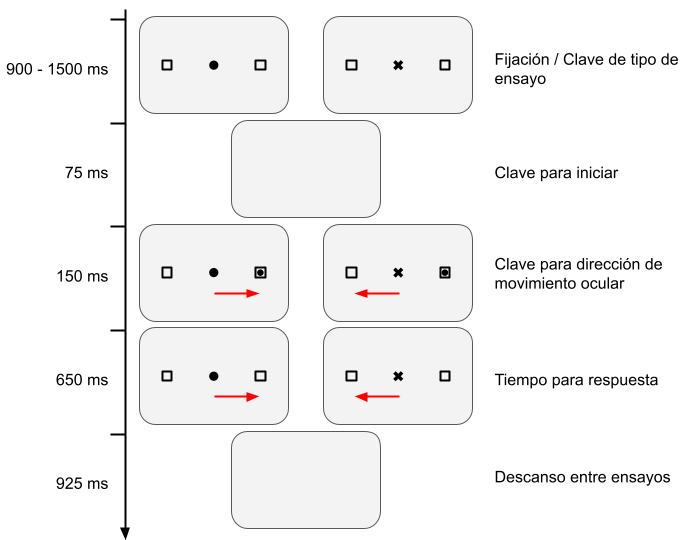
\includegraphics[width=0.8\linewidth]{media/antisaccades-protocol.png}}

    El sujeto sabrá si está ante un ensayo de antisacadas o de prosacadas según
    la forma del estímulo central de fijación.
    Un círculo representa un ensayo de prosacadas mientras que una cruz
    representa un ensayo de antisacadas.
    El estímulo lateral fue representado con un círculo.
    Las duraciones de cada fase se eligieron entre los rangos encontrados en
    otros protocolos.
    Con el fin de evitar que entrara en juego la memoria visual espacial,
    fueron dibujadas cajas sobre las posiciones en las cuales aparecerían los
    estímulos laterales.

    \caption{Protocolo de la tarea de antisacadas}
    \label{fig:antisaccades-protocol}
  \end{figure}

  La calibración del sistema fue basada en aquellas encontradas en otros
  \eyetrackers, ya sean \eyetrackers comerciales (\tobii, \eyelink) o trabajos
  recientes de \eyetracking web \cite{xu_2015_turker_gaze,
  papoutsaki_2016_webgazer}.
  En ella el sujeto tendrá que fijar la mirada en una secuencia de estímulos,
  presionando la barra de espacio cada vez que lo hiciera (figura
  \ref{fig:calibration-protocol}).
  La validación luego de cada calibración siguió las mismas líneas.
  Para cada uno de estos estímulos presentados se selecciona el frame anterior a
  la interacción del sujeto.
  El frame es luego asociado a la coordenada del estímulo presentado.

  \begin{figure}
    \centering

    Ejemplos de estímulos de calibración:

    \includegraphics[width=0.4\linewidth]{media/calibration-stimulus-left.png}
    \includegraphics[width=0.4\linewidth]{media/calibration-stimulus-center.png}
    \includegraphics[width=0.4\linewidth]{media/calibration-stimulus-right.png}

    Los estímulos presentados son círculos negros en coordenadas específicas de
    la pantalla.
    Durante cada fase de calibración, el sujeto es presentado en total con 11
    de ellos.
    9 de ellos se alinean sobre el eje medio horizontal, 3 de ellos en cada
    región de interés (izquierda, centro y derecha).
    Otros 2 se muestran sobre el eje central vertical, uno en el bloque
    superior y otro en el bloque inferior.
    La fijación en el estímulo es indicada mediante una interacción con el
    navegador web, puntualmente con un presionado de la barra de espacio.

    \caption{Protocolo de calibración}
    \label{fig:calibration-protocol}
  \end{figure}

  Tanto la tarea de antisacadas como la rutina de calibración fueron
  implementadas en compatibilidad con \jspsych y utilizando su \textit{plugin}
  \psychophysics para dibujar estímulos.

  En ambos experimentos tuvo que considerarse su duración total al momento de 
  elegir la cantidad de ensayos que serían presentados a cada sujeto.
  En la primera ronda se apuntó a una duración cercana a los 10 minutos.
  Fallas intermitentes de \webgazer causaban \crashes del prototipo implementado
  o incluso de la pestaña en uso del navegador.
  Estas fallas ya habían sido reportadas por octubre de 2020 en el repositorio
  original \footnote{reporte inicial de falla:
  \url{https://github.com/brownhci/WebGazer/issues/171}} pero a falta de
  respuesta se lo reportó también a la comunidad de JSPsych \footnote{segundo
  reporte: \url{https://github.com/jspsych/jsPsych/discussions/2490}}.
  Para la segunda instancia en base a este mismo trabajo y modificaciones sobre
  \webgazer, tal falla había sido resuelta.
  En consecuencia se estiró la duración del experimento a entre 20 y 25 minutos.

  Durante la primera ronda el sujeto fue presentado únicamente con ensayos de
  antisacadas.
  Cada sujeto realizó 160 ensayos de ella, distribuidos en 10 de prueba seguidos
  de 3 bloques de 50 ensayos cada uno.
  Luego de cada ensayo en el cual se detectara una descalibración, se prosiguió
  a una calibración del sistema.
  En la segunda ronda se realizaron tanto antisacadas como prosacadas.
  Cada sujeto debió realizar 160 ensayos de cada tarea, estos distribuidos en
  bloques intercalados de 20 ensayos, sumado a 10 ensayos iniciales de prueba
  para cada tarea.
  En esta instancia se dió también la opción de cortar tempranamente a la mitad
  del experimento en caso de que el sujeto se hubiera cansado luego de la primera
  mitad.
  A diferencia de la ronda anterior, en esta se calibró únicamente al final de
  cada bloque.
  Además se agregó una fase de validación posterior a cada calibración.

  Los experimentos fueron distribuidos a través de las plataformas \cognition
  (\url{https://www.cognition.run/}) y \neuropruebas
  (\url{https://neuropruebas.org/}).
  Se informó a los sujetos sobre la posibilidad de realizar los experimentos a
  través de redes sociales, del \textit{mailing list} provisto por \neuropruebas
  y de círculos privados de familiares y amigos.
  Los sujetos fueron informados sobre cómo sería utilizada su cámara web.
  Entre quienes hubieran realizado el experimento a través de \neuropruebas se 
  realizaron sorteos por libros del gato y la caja
  (\url{https://twitter.com/liaa_icc/status/1528028122465058816}).

\subsection{Prototipo de estimación de la mirada aplicado a estudios clínicos}

  El prototipo implementado para cubrir el rol de eye tracker web nació de
  estudiar la posibilidad del paquete \webgazer en cumplir nuestros objetivos.
  Este paquete provee los bloques elementales para realizar estimación de la
  mirada.
  Incluye \begin{enumerate*}
    \item localización de los ojos (figura \ref{fig:eyes-localization}),
    \item traducción de los recuadros de los ojos a la entrada del modelo
      interno de regresión lineal \textit{ridge} (figura
      \ref{fig:eye-features-to-model-input}) y
    \item emisión de estimaciones sobre la coordenada observada en la pantalla
      a través de tal modelo
  \end{enumerate*}.
  Las especificaciones del software que nos iba a ser necesario no estaban
  claras inicialmente, sino que fueron estableciendose a medida que el trabajo
  avanzaba.
  Entre otros, se denotó la ausencia de una rutina de calibración adecuada a
  nuestro protocolo y de un mecanismo de detección de descalibración del
  sistema.
  El software resultante, sumado al código de los experimentos y al código de
  análisis de datos, fue liberado en un repositorio público \footnote{
    repositorio principal:
    \url{https://github.com/ffigari/rastreador-ocular}
  }.
  Los cambios realizados sobre \webgazer pueden consultarse en un \fork
  personal de paquete \footnote{
    \fork propio:
    \url{https://github.com/ffigari/WebGazer}
  }.
  Para este \fork no se partió del repositorio original de \webgazer \footnote{
    repositorio original:
    \url{https://github.com/brownhci/WebGazer}
  } sino del \fork realizado por \jspsych \footnote{
    \fork de \jspsych:
    \url{https://github.com/jspsych/WebGazer}
  }.
  La razón de esto fue maximizar las chances de mantener compatibilidad con
  \jspsych.

  \begin{figure}
    \centering
    \begin{verbatim}
    def localizar-ojos(frame):
        en base al frame de entrada
        generar
          el facemesh f
          correspondiente a la salida del modelo de facemesh

        para cada ojo
        definir
          la región de interés
          ri = area entre ambos párpados y ambas comisuras
        
        de la salida del modelo de facemesh f
        seleccionar
          los conjuntos
          as, ai = keypoints correspondientes a
                   los arcos superior e inferior de ri
        
        para cada ojo
        calcular
          la esquina superior izquierda
          esi = mínimos x y entre las coordenadas de as
        calcular
          la esquina inferior derecha
          eid = máximos x y entre las coordenadas de ai
      
        retornar para cada ojo
          el recuadro
          definido por las esquinas esi y eid\end{verbatim}

    Los recuadros devueltos por esta rutina son de dimensión variable.
    Además asume que una y sólo una cara será detectada por el modelo de
    \facemesh.
    El modelo de \tfjs utilizado da la opción de detectar una única cara.
    Es sin embargo posible, aunque sea por la valida razón de que nadie se
    encuentre sentado frente a la webcam, que en algún \textit{frame} no se
    detecte ninguna cara.
    El resto del programa tiene que tener en cuenta esta posibilidad.
    \caption{Localización de los ojos}
    \label{fig:eyes-localization}
  \end{figure}

  \begin{figure}
    \begin{verbatim}
    def generar-input-de-webgazer(recuadros):
        llevar cada recuadro
        a un vector
          de dimensión fija de 6 píxeles de alto y 10 píxeles de ancho
          en escala de grises
          y ecualizado por histograma

        retornar la concatenación de ambos vectores\end{verbatim}
    El vector resultante tendrá 120 dimensiones.
    Esta rutina es un ejemplo de modelado por apariencia.
    \caption{Generación de entrada del modelo de estimación de la mirada}
    \label{fig:eye-features-to-model-input}
  \end{figure}

  El sistema resultante nace en la localización \textit{frame} a \textit{frame}
  de los ojos (figura \ref{fig:eyes-localization})
  \footnote{
    La localización de los ojos de \webgazer tuvo que ser modificada para
    resolver la falla que limitó temporalmente la primera ronda de
    experimentación.
    Para lograrlo fue necesario reemplazar el paquete utilizado para la
    generación del \facemesh
    (\url{https://github.com/ffigari/WebGazer/commit/e5df9f9c3521ec3e384e962db49d94b2411789bb}).
    Aquel de la versión original de \webgazer era
    \texttt{@tensorflow-models/facemesh}
    (\url{https://www.npmjs.com/package/@tensorflow-models/facemesh}) pero este
    paquete se encontraba deprecado.
    Siguiendo la sugerencia de ese mismo paquete, se lo reemplazó por
    \texttt{@tensorflow-models/face-landmarks-detection}
    (\url{https://www.npmjs.com/package/@tensorflow-models/face-landmarks-detection}).
    Tal reemplazo implicó retrabajar cómo se seleccionaba el recuadro del ojo
    en base a la salida del modelo de \facemesh.
    Esta modificación fue luego \mergeada en el repositorio original de
    \webgazer
    (\url{https://github.com/brownhci/WebGazer/commit/96ecaa8b84a5d09ba4f0bcf5c4000a0bc3623f0a}).
    Resolver esta falla fue la principal motivación detrás de las otras mejoras
    realizadas.
  }.
  Al localizar los ojos, se calculan \features sobre ellos.
  Estas contienen el parche del \textit{frame} seleccionado por la rutina de
  localización de los ojos (almacenado en un objeto \texttt{ImageData}
  \footnote{
    documentación de \texttt{ImageData}:
    \url{https://developer.mozilla.org/en-US/docs/Web/API/ImageData}
  } equivalente a una matriz con la información de cada píxel), sus dimensiones
  y la coordenada de su esquina superior izquierda, todos valores en píxeles.
  La frecuencia de generación de estos \features está sujeta a \raf que a su
  vez está sujeto a la tasa de refresco del monitor \footnote{
    documentación de \raf:
    \url{https://developer.mozilla.org/en-US/docs/Web/API/window/requestAnimationFrame}
  }.
  Estas \features son propagadas al contexto global del navegador a través de
  eventos de \js de navegador \footnote{
    documentación sobre \texttt{CustomEvent}:
    \url{https://developer.mozilla.org/en-US/docs/Web/API/CustomEvent/CustomEvent}
  }.
  Esto no ocurría originalmente, sino luego de un cambio necesario para poder
  reutilizarlas en la detección de movimiento \footnote{
    propagación de \features:
    \url{https://github.com/ffigari/WebGazer/commit/7c6b7fb4dcefea2b85d7a24b3e86bd9a31b938d4}
  }.

  En cada instante de calibración se notifica a \webgazer para que transforme
  el último par de \features al formato necesario a su modelo de regresión
  (figura \ref{fig:eye-features-to-model-input}) y la almacene junto a la
  coordenada del estímulo presentado.
  Además, se almacenan los recuadros correspondientes a las posiciones de los
  ojos.
  En base a los datos recolectados, al finalizar la fase de calibración se
  notifica finalmente a \webgazer para que instancie su modelo de regresión
  \footnote{
    La instanciación del modelo de regresión de \webgazer estuvo sujeta a
    cambios
    (\url{https://github.com/ffigari/WebGazer/commit/16f69474d40132c7faa826b2afc7fd464bc6c6c5}).
    Originalmente \webgazer permitía agregar datos de calibración en cualquier
    momento durante el ciclo de vida del estimador de la mirada.
    Sin embargo esto implicaba recalcular en cada \textit{frame} los
    coeficientes del modelo interno de regresión, mientras que para nuestro
    caso alcanzaba con calcularlos al final de la fase explícita de
    calibración.
    Al ser esto una optimización de recursos, se optó por modificar \webgazer y
    su interfaz para que el calculo de coeficientes se realice a través de un
    pedido explícito.
  }

  Al finalizar la calibración se instancia además la detección de movimiento.
  Los recuadros almacenados definen a su vez una región de ``quietud'' (figura
  \ref{fig:features-to-stillness-region}) dentro de la cual tendrán que estar
  contenidos los recuadros subsecuentes.
  Si en algún \textit{frame} alguno de los recuadros sale de tal región
  entonces se considerará que el sujeto se movió (figura
  \ref{fig:movement-detection}).
  Cuando esto suceda se considerará y notificará que el sistema ha pasado a 
  estar descalibrado.

  \begin{figure}
    \begin{verbatim}
    def definir-region-de-quietud(recuadros):
        para cada ojo
        definir
          su región de quietud
          q = la unión
              de sus recuadros
              agrandados por un factor de 1.8

        retornar ambas regiones de quietud\end{verbatim}
    Los recuadros de cada ojo son representados con rectángulos y cada
    región de quietud con un ``multirectángulo'' (\ie, la unión de varios
    rectángulos).
    La elección del valor de este factor impacta posteriormente en el rigor de
    la detección.
    \caption{Definición de regiones de quietud}
    \label{fig:features-to-stillness-region}
  \end{figure}

  \begin{figure}
    \begin{verbatim}
    def detectar-movimiento(par de regiones de quietud):
        cada vez que sea propagado un par de features de los ojos
          para cada feature
          verificar que esta esté contenida en su región de quietud

        si alguno de los dos features
        no estuviera contenido en su región de quietud
        entonces notificar que se detectó movimiento\end{verbatim}
    \caption{Detección de movimiento}
    \label{fig:movement-detection}
  \end{figure}

  La detección de descalibraciones no interrumpirá la generación de
  estimaciones de la mirada.
  En cambio, el protocolo experimental será aquel que defina cómo lidiar con
  las descalibraciones y cuándo proceder a una nueva calibración del sistema.

  Con la implementación presentada se apuntó a mantener compatibilidad con
  \jspsych.
  En paralelo se busco minimizar las dependencias a tal \framework.
  Para esto se distinguieron dos interfaces lógicas:
  \begin{enumerate}
    \item
      La externa, que proveyendo \timelines de \jspsych apunta a facilitar la
      implementación de experimentos clínicos que requieran \eyetracking.
      Durante el \runtime de un experimento, estos permiten calibrar el
      sistema, validar tal calibración y realizar recalibraciones si fuera
      necesario.
    \item
      La interna, que provee lo esencial al funcionamiento.
      Esto incluye la interacción con \webgazer y el seguimiento del estado de
      calibración.
  \end{enumerate}
  En base a esta distinción se implementaron dos \playgrounds, los cuales son
  interfaces web que permiten interactuar con cada interfaz lógica (figuras
  \ref{fig:external-playground} y \ref{fig:internal-playground}).
  Estos facilitan el desarrollo de cada interfaz lógica y por lo tanto de todo
  el prototipo.
  La interfaz externa permite calibrar el sistema utilizando el protocolo ya
  mencionado durante el cual se dibujan estímulos en la pantalla.
  Además, ambas interfaces permiten calibrar libremente.
  Esto consiste en generar datos de calibración a partir de clicks en la
  pantalla durante los cuales se deberá fijar la mirada en el puntero.

  \begin{figure}
    \centering
    \frame{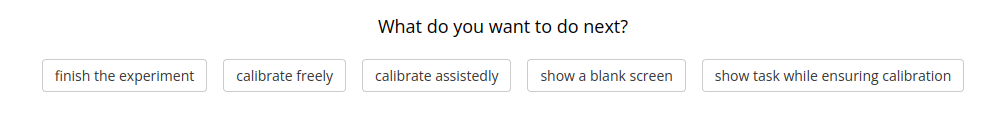
\includegraphics[width=0.8\linewidth]{metodo/external-playground.png}}

    Se puede elegir entre:
    a) calibrar libremente;
    b) calibrar asistidamente;
    c) mostrar un HTML básico mientras se estima la mirada;
    d) realizar una secuencia de ensayos de una tarea de juguete mientras
    entre ensayos se asegura la correcta calibración del sistema;
    e) finalizar la sesión para exportar la data recolectada.

    \caption{\textit{Playground} externo}
    \label{fig:external-playground}
  \end{figure}

  \begin{figure}
    \centering
    \frame{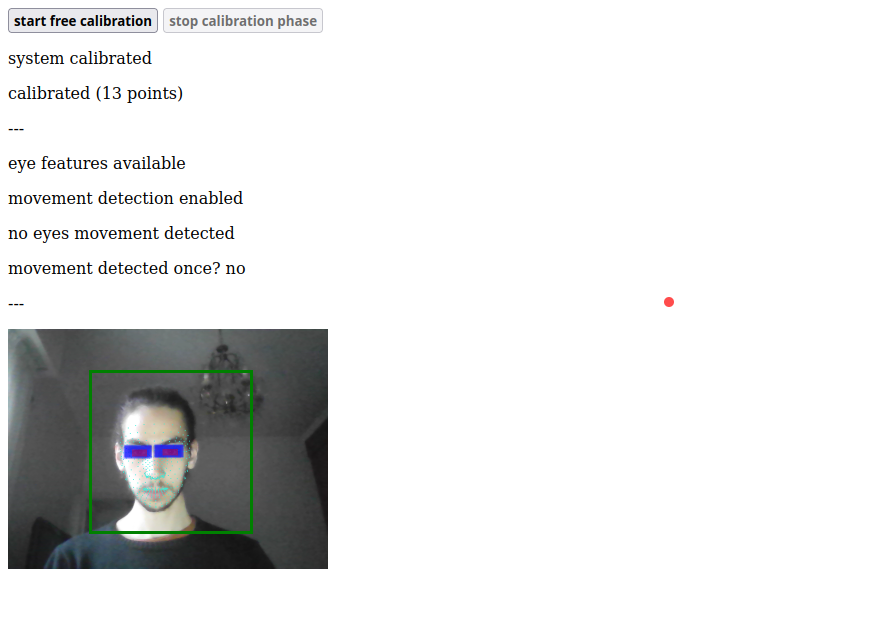
\includegraphics[width=0.8\linewidth]{metodo/internal-playground.png}}

    Información del estado del \eyetracker es presentada al mismo tiempo que se
    permite realizar calibraciones libres.
    El recuadro verde corresponde a la posición dentro de la cual el paquete
    \webgazer exige que aparezca la cabeza, los rectángulos rojos corresponden
    a los recuadros de los ojos en cada \textit{frame} y los rectángulos azules
    corresponden a las posiciones dentro de las cuales los recuadros de los
    ojos deben mantenerse para considerar que no hubo movimiento.
    El punto rojo correspode a la posición estimada de la mirada.

    \caption{\textit{Playground} interno}
    \label{fig:internal-playground}
  \end{figure}

\subsection{Extracción de información}

  La experimentación realizada permitió obtener estimaciones de la mirada para
  múltiples ensayos provenientes de múltiples sujetos, tanto para la tarea de
  antisacadas como para la tarea de prosacadas.
  Con el análisis posterior se buscó principalmente aislar la respuesta dada en
  cada ensayo ante la aparición del estímulo visual lateral, así como la
  latencia en dar tal respuesta.
  Para ello se aplicaron rutinas \adhoc de detección de sacadas para encontrar
  la dirección y el inicio de la primera sacada en cada ensayo si esta
  existiera.
  Previo a esto se descartaron datos que se consideraran inválidos.
  Los datos conservados fueron normalizados a un rango común de valores debido
  a las desviaciones encontradas en los datos (figura
  \ref{fig:skewed-estimations-example}) y su variabilidad en cuanto a
  frecuencias de muestreo y resoluciones de pantalla (figuras
  \ref{fig:first-starting-sample-distribution} y
  \ref{fig:second-starting-sample-distribution}).
  El análisis de datos implementado ignoró el eje vertical (\ie, la coordenada
  ``y'' de cada estimación) pues no interesaba a nuestro objeto de estudio.

  \begin{figure}
    \centering

    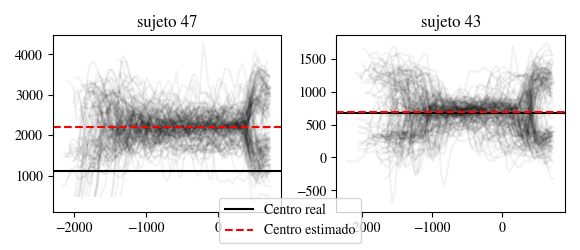
\includegraphics[width=\textwidth]{metodo/skewed-estimations-examples.png}

    Durante la fase de fijación los sujetos 47 y 24 obtuvieron respectivamente
    estimaciones cercanas a los 2100 y 1400 píxeles cuando los valores reales
    serían 1100 y 900.
    Estas desviaciones no ocurrieron para todo sujeto, como lo muestran los
    sujetos 43 y 22. \\
    Las estimaciones mantienen sin embargo un correcto posicionamiento
    relativo.
    Por lo tanto pueden utilizarse para extrapolar data a pesar de las
    desviaciones.

    \caption{Ejemplos de sujetos con estimaciones desviadas}
    \label{fig:skewed-estimations-example}
  \end{figure}

  El primer punto que se atacó fue la variabilidad de la frecuencia de
  muestreo.
  Para esto se realizó un remuestreo de las estimaciones de todo ensayo a 30
  Hz.
  Esto se hizo utilizando interpolación lineal \footnote{
    interpolación lineal:
    \url{https://es.wikipedia.org/wiki/Interpolaci\%C3\%B3n\_lineal}
  }.

  Las estimaciones fueron luego normalizadas tal que el valor $0$ se
  correspondiera con la posición de fijación.
  Para la primera ronda se calculó para cada sujeto el promedio de la
  coordenada ``x'' estimada durante la fase de fijación de cada ensayo.
  A las estimaciones de los ensayos de cada sujeto se sustrajo luego tal valor
  con el fin de centrarlos alrededor del $0$.
  Cada ensayo fue luego llevado al rango $[-1, 1]$ tal que aproximadamente $-1$
  se correspondiera al valor mínimo del ensayo y $1$ al valor máximo.

  Para la segunda ronda se normalizó en base a las validaciones realizadas
  luego de cada calibración.
  En estas validaciones, las coordenadas de los estímulos laterales presentados
  coincidieron con las coordenadas de los estímulos visuales laterales de las
  tareas de pro y antisacadas.
  Para cada ensayo se tomó entonces la última validación y se calcularon los
  valores $l$, $c$ y $r$ correspondientes respectivamente al promedio de las
  estimaciones durante la presentación de los estímulos a la izquierda, al
  centro y a la derecha.
  Luego, las estimaciones en el rango $[l, c]$ fueron llevadas al rango $[-1,
  0]$ y aquellas en el rango $[c, r]$ al rango $[0, 1]$.

  Luego de normalizar las estimaciones se espejó la mitad de ellas tal que
  pudiera asumirse que el estímulo visual lateral aparecía siempre del mismo
  lado.
  El espejado se realizó multiplicando por $-1$ las estimaciones de los ensayos
  en los cuales el estímulo lateral apareciera a izquierda.
  Esto no era estrictamente necesario, pero simplificó análisis posteriores.
  Luego de este cambio, toda antisacada correcta tendrá que mostrar en sus
  estimaciones un salto de un valor cercano a $0$ a un valor cercano a $-1$.
  Similarmente, toda prosacada correcta tendrá que mostrar un salto hacia los
  valores negativos.
  La figura \ref{fig:normalization-looks-example} ejemplifica las
  transformaciones ocurridas en las estimaciones al normalizarlas.

  \begin{figure}
    \centering

    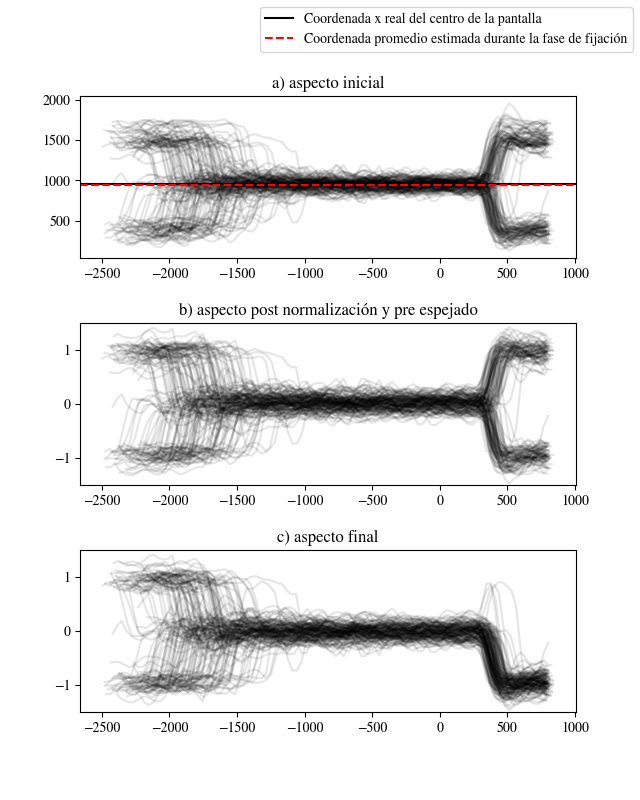
\includegraphics[width=\linewidth]{metodo/normalization-looks-example.png}

    Se muestran las estimaciones de los ensayos de antisacadas para el sujeto
    44 de la segunda instancia.

    \caption{Cambios en el aspecto de las estimaciones al normalizarlas}
    \label{fig:normalization-looks-example}
  \end{figure}

  Se buscó luego descartar aquellos ensayos donde no pudiera determinarse una
  respuesta por parte del sujeto ya fuera esta correcta o incorrecta.
  Así, se clasificó como \outlier a todo ensayo en el cual:
  \begin{itemize}
    \item la frecuencia original de muestreo fuera menor a 15 Hz
    \item no hubiera habido fijación en el estímulo central durante los 500 ms
      anteriores a la aparición del estímulo lateral
    \item hubiera una sacada temprana antes de los 100 ms posteriores a la
      aparición del estímulo lateral
    \item no hubiera sacada
  \end{itemize}
  Para algunos sujetos la totalidad de sus datos fue manualmente marcada como
  \outlier.
  Los \outliers fueron luego descartados, así como todas las estimaciones de
  los sujetos que terminaran con menos de 30 ensayos luego de haber aplicado
  los criterios de filtrado anteriores.

  Los ensayos no descartados definieron el grupo \inlier, grupo sobre el cual
  se reportarán luego las tasas de correctitud y las latencias en las
  respuestas.

  La detección de sacadas de la primera ronda se implementó en base a detectar
  cuándo las estimaciones post normalización cruzaban los umbrales $0.6$ o
  $-0.6$ indicando respectivamente una sacada hacia el estímulo o en dirección
  contraria.

  En la segunda instancia se buscó aplicar elementos comunmente utilizados en
  la bibliografía.
  Para ello post normalización se clasificó como sacada a los intervalos que
  \begin{enumerate*}
    \item duraran al menos 40 ms,
    \item tuvieran estimaciones monotónicamente crecientes o decrecientes,
    \item hubieran recorrido al menos 0.6 unidades y
    \item tuvieran una velocidad promedio de al menos 0.15 unidades / 100 ms
  \end{enumerate*}.
